\chapter{Compact Surfaces}
\section{Surfaces}
A surface is a $2$-manifold. We have already seen several important examples of
compact surfaces: the sphere $S^2$, the torus $T^2$, and the projective plane $\P^2$.\par
In order to systematize our knowledge of surfaces, it is useful to develop a uniform way to represent them as CW complexes. The prototype is the representation
of the torus as a quotient of the square by identifying the edges in pairs. It turns out that every compact surface can be represented as a quotient of a polygonal region in the plane by an equivalence relation that identifies its edges in pairs.
\begin{example}
The sphere $S^2$ is homeomorphic to the following quotient spaces.
\begin{itemize}
\item The closed disk $\widebar{\B}^2\sub\R^2$ modulo the equivalence relation generated by $(x,y)\sim(-x,y)$ for $(x,y)\in\partial\B^2$.
\item The square region $S=\{(x,y)\mid |x|+|y|\leq 1\}$ modulo the equivalence relation generated by $(x,y)\sim(-x,y)$ for $x\in\partial S$.
\end{itemize}
\end{example}
\begin{example}
The projective plane $\P^2$ is homeomorphic to each of the following quotient spaces
\begin{itemize}
\item The closed disk $\widebar{\B}^2$ modulo the equivalence relation generated by $(x,y)\sim(-x,y)$ for $(x,y)\in\partial\B^2$.
\item The square region $S=\{(x,y)\mid |x|+|y|\leq 1\}$ modulo the equivalence relation generated by $(x,y)\sim(-x,-y)$ for $x\in\partial S$.
\end{itemize}
\end{example}
Now we describe a general method for building surfaces by identifying edges of
geometric figures. We define a \textbf{polygon} to be a subset of $\R^2$ that is homeomorphic to $S^1$ and is the union of \textbf{finitely many} $1$-simplices that meet only at their endpoints; thus it is the polyhedron of a $1$-dimensional simplicial complex, and a regular finite CW complex. The $0$-simplices and $1$-simplices of the polygon are called its \textbf{vertices}
and \textbf{edges}, respectively. It follows from Lemma~\ref{one mani 0-cell 1-cell} that each vertex lies on exactly two edges.\par
Then we define a \textbf{polygonal region} to be a compact subset of $\R^2$ whose interior is a regular coordinate ball (and thus a regular $2$-cell), and whose boundary is a polygon. The edges and vertices of the boundary polygon are also referred to as the edges and vertices of the polygonal region. Any $2$-simplex in the plane is easily seen to be a polygonal region, as is a filled-in square, or any compact convex region that has a nonempty interior and polygonal boundary. Below, we will see more examples of manifolds obtained as quotients of polygonal regions by identifying the edges in pairs. It is a general fact that such a quotient space is always a surface.
\begin{proposition}\label{polygonal quotient}
Let $P_1,\cdots,P_k$ be polygonal regions in the plane, let $P=\coprod_{i=1}^kP_i$, and suppose we are given an equivalence relation on $P$ that identifies some of the edges of the polygons with others by means of affine homeomorphisms.
\begin{itemize}
\item[$(a)$] The resulting quotient space is a finite $2$-dimensional CW complex whose $0$-skeleton is the image under the quotient map of the set of vertices of $P$, and whose $1$-skeleton is the image of the union of the boundaries of the polygonal regions.
\item[$(b)$] If the equivalence relation identifies each edge of each $P_i$ with exactly one other edge in some $P_j$ $($which might or might not be equal to $P_i$ $)$, then the resulting quotient space is a compact $2$-manifold.
\end{itemize}
\end{proposition}
\begin{proof}
Let $M$ be the quotient space, let $\pi:P\to M$ denote the quotient map, and let $M_0$, $M_1$, and $M_1=M$ denote the images under $\pi$ of the vertices, boundaries, and polygonal regions, respectively. It follows easily from the definition that $M_0$ is discrete, and for $k=1,2$, $M_k$ is obtained from $M_{k-1}$ by attaching finitely many $k$-cells. Thus $(a)$ follows from Theorem~\ref{CW construction}.\par
Now assume the hypothesis of $(b)$. By Proposition~\ref{CW comp into mani}, to prove that $M$ is a manifold, it suffices to show that it is locally Euclidean.
Because the $2$-cells are open in $M$, they are Euclidean neighborhoods of each
of their points. Thus it suffices to show that each point in a $1$-cell or a $0$-cell has a Euclidean neighborhood.\par
A point $q$ in a $1$-cell has exactly two preimages $q_1$ and $q_2$, each in the interior of a different edge. Since each $P_i$ is a $2$-manifold with boundary, and 
$q_1,q_2$ are boundary points, each $q_i$ has a neighborhood $U_i$ that is a regular coordinate halfball. By shrinking the neighborhoods if necessary, we may assume 
that the equivalence relation identifies the boundary segment of $U_1$ exactly with that of $U_2$. Then the same argument as in Theorem~\ref{adju mani} shows that 
$q$ has a Euclidean neighborhood.\par
The preimage of a $0$-cell $v$ is a finite set of vertices $\{v_0,\cdots,v_k\}\sub P$. For each of these vertices, we can choose $\eps$ small enough that the disk $\B(v_i,\eps)$ contains no vertices other than $v_i$, and intersects no edges other than the two that have $v_i$ as endpoints. Because the interior of the polygonal region $P_j$ of which $v_i$ is a vertex is a regular coordinate ball, it lies on one side of its boundary, so $\B(v_i,\eps)\cap P_j$ is equal to a wedge defined by the intersection of two closed half-planes whose boundaries intersect only at $v$. It is then easy to construct a homeomorphism from $\B(v_i,\eps)\cap P_j$ to a wedge of angle $2\pi/k$, which is a set described in polar coordinates by $\{(r,\theta):\theta_0\leq\theta\leq\theta_0+2\pi/k\}$. (If we place $v_i$ at the origin, such a homeomorphism is given in polar coordinates by a map of the form $(r,\theta)\mapsto(r,\theta_0+c\theta)$ for suitable constants $\theta_0$, $c$. Such a map is sometimes called a \textbf{fan transformation}, because it suggests the opening or closing of a folding paper fan.)
\[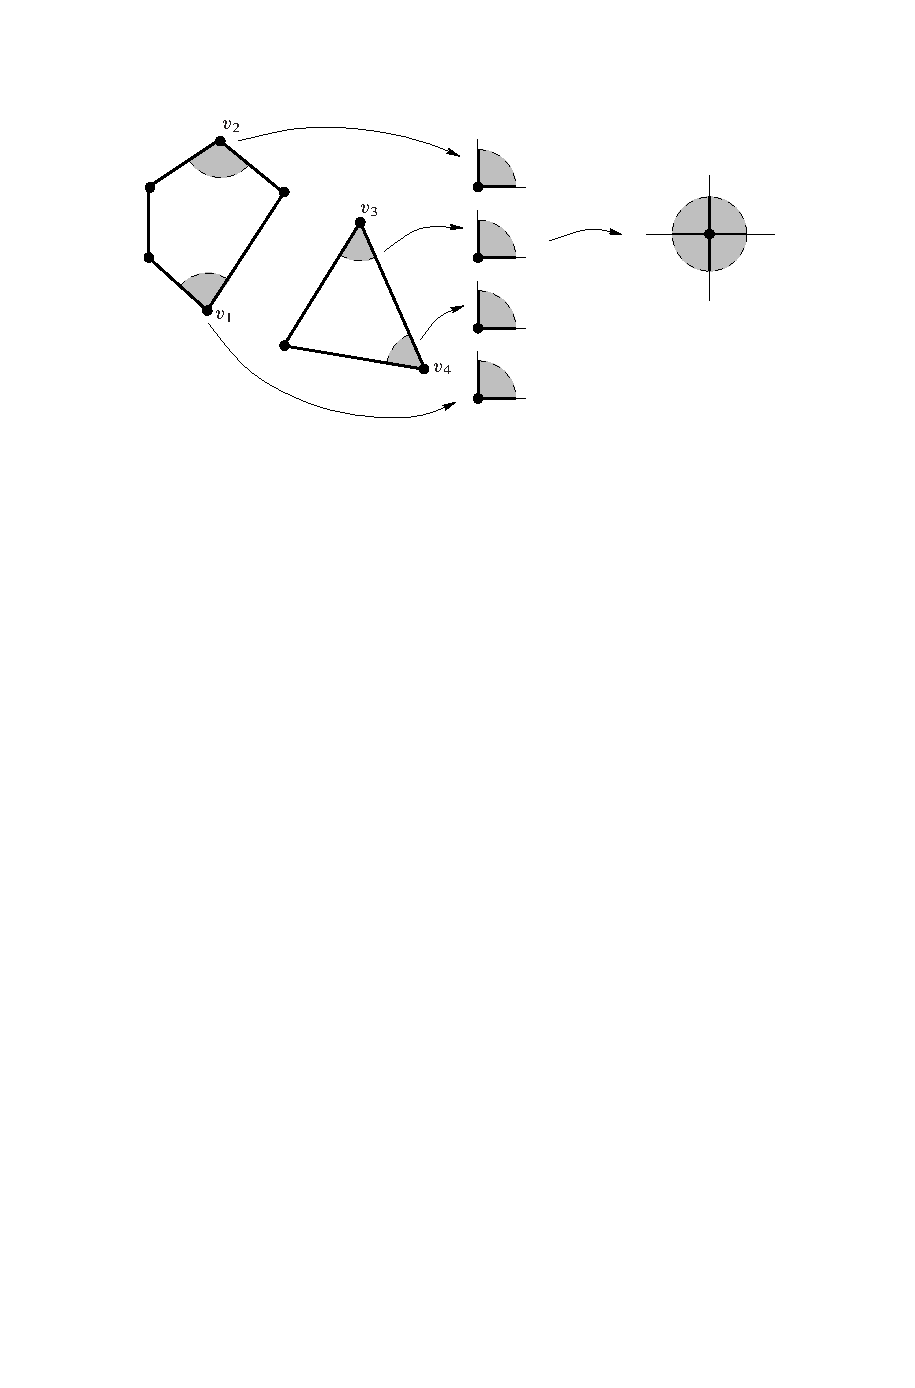
\includegraphics{Euclidean-neighborhood-of-vertex-point.pdf}\]
Because each edge is paired with exactly one other, the $k$ wedges can be mapped
onto a set containing a neighborhood of the origin by rotating and piecing them
together. However, this may not respect the edge identifications. To correct this,
we can subject each wedge to a preliminary transformation that rescales its edges independently. First, by a rotation followed by a fan transformation, take the wedge to the first quadrant so that one edge lies along the positive $x$-axis and the other along the positive $y$-axis. Then rescale the two axes by a linear transformation $(x,y)\mapsto(ax,by)$. Finally, use another fan transformation to insert the wedge into its place. (The case $k=1$ deserves special comment. This case can occur only if the two edges adjacent to the single vertex $v_1$ are identified with each other; then you can check that our construction maps a neighborhood of $v_1$ onto a neighborhood of the origin, with both edges going to the same ray.) In each case, we end up with a map defined on a saturated open subset of $P$, which descends to a homeomorphism from a neighborhood of $v$ to a neighborhood of the origin in $\R^2$.\par
The compactness comes from Theorem~\ref{CW compact iff}.
\end{proof}
\begin{example}
The \textbf{Klein bottle} is the $2$-manifold $K$ obtained by identifying the edges of the square $I\times I$ according to $(0,t)\sim(1,t)$ and $(t,0)\sim(1-t,1)$ for $0\leq t\leq1$. To visualize $K$, think of attaching the left and right edges together to form a cylinder, and then passing the upper end of the cylinder through the cylinder wall near the lower end, in order to attach the upper circle to the lower one from the inside. Of course, this cannot be done with a physical model; in fact, it can be shown that the Klein bottle is not homeomorphic to any subspace of $\R^3$. Nonetheless, the preceding proposition shows that it is a $2$-manifold.
\[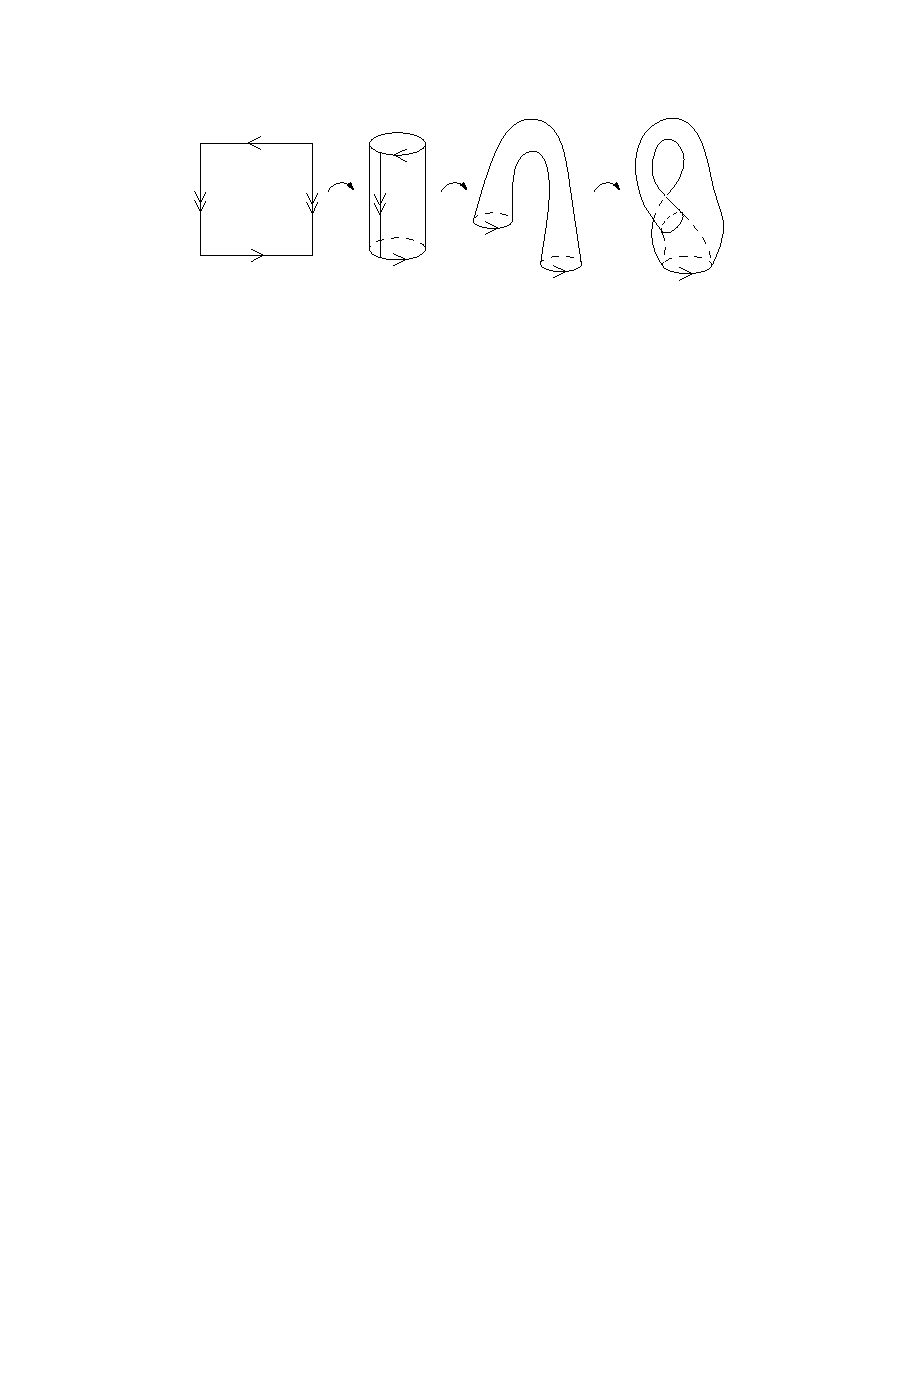
\includegraphics{Klein-bottle.pdf}\]
\end{example}
\section{Connected Sums of Surfaces}
Given connected $n$-manifolds $M_1$ and $M_2$ and regular coordinate balls $B_i\sub M_i$, the subspaces $M'_i=M_i\setminus B_i$ are $n$-manifolds with boundary whose boundaries are homeomorphic to $S^{n-1}$. If $f:\partial M'_2\to\partial M'_1$ is any homeomorphism, the adjunction space $M'_1\cup_fM'_2$ is denoted by $M_1\#M_2$ and is called a connected sum of $M_1$ and $M_2$. $M_1\#M_2$ is a connected $n$-manifold.\par
The manifold $M_1\#M_2$ depends on several choices: the sets $B_i$ and the homeomorphism $f$. Although we will not prove it, it can be shown that it is possible to obtain at most two nonhomeomorphic manifolds as connected sums of a given pair $M_1$ and $M_2$. (The two possibilities correspond to the cases in which $f$ preserves or reverses the orientation of the sphere.)
\begin{example}
If $M$ is any $n$-manifold, a connected sum $M\#S^n$ is homeomorphic to $M$, at least if we make our choices carefully. Let $B_2\sub S^n$ be the open lower hemisphere, so $(S^n)'=S^n\setminus B_2$ is the closed upper hemisphere, which is
homeomorphic to a closed ball. Then $M\#S^n$ is obtained from $M$ by cutting out the open ball $B_1$ and pasting back a closed ball along the boundary sphere, so we have not changed anything.
\end{example}
\begin{example}
A connected sum of a $2$-manifold $M$ with $T^2$ can be viewed in another way, as a space obtained by \textbf{attaching a handle} to $M$. To make this precise, let 
$M_0$ denote $M$ with two regular coordinate disks removed. Then $M_0$ and $S_1\times I$ are both manifolds with boundary, and each boundary is homeomorphic to a 
disjoint union of two circles. Let $\widetilde{M}$ be the adjunction space obtained by attaching $M_0$ and $S_1\times I$ together along their boundaries 
(Theorem~\ref{adju mani}). The reason this quotient space is homeomorphic to $M\#T^2$ is suggested in the figure below, which shows that a space homeomorphic to 
$M\#T^2$ can also be obtained by first removing the interior of a regular coordinate disk from $M$, then attaching a closed disk with two open disks removed, and then 
finally attaching the cylinder $S^1\times I$ along the two remaining boundary circles. Since the first operation results in a space homeomorphic to $M$ with two regular 
coordinate disks removed, the result is the same as if we had started by removing two disks and then attached the cylinder to the two resulting boundary circles.
\[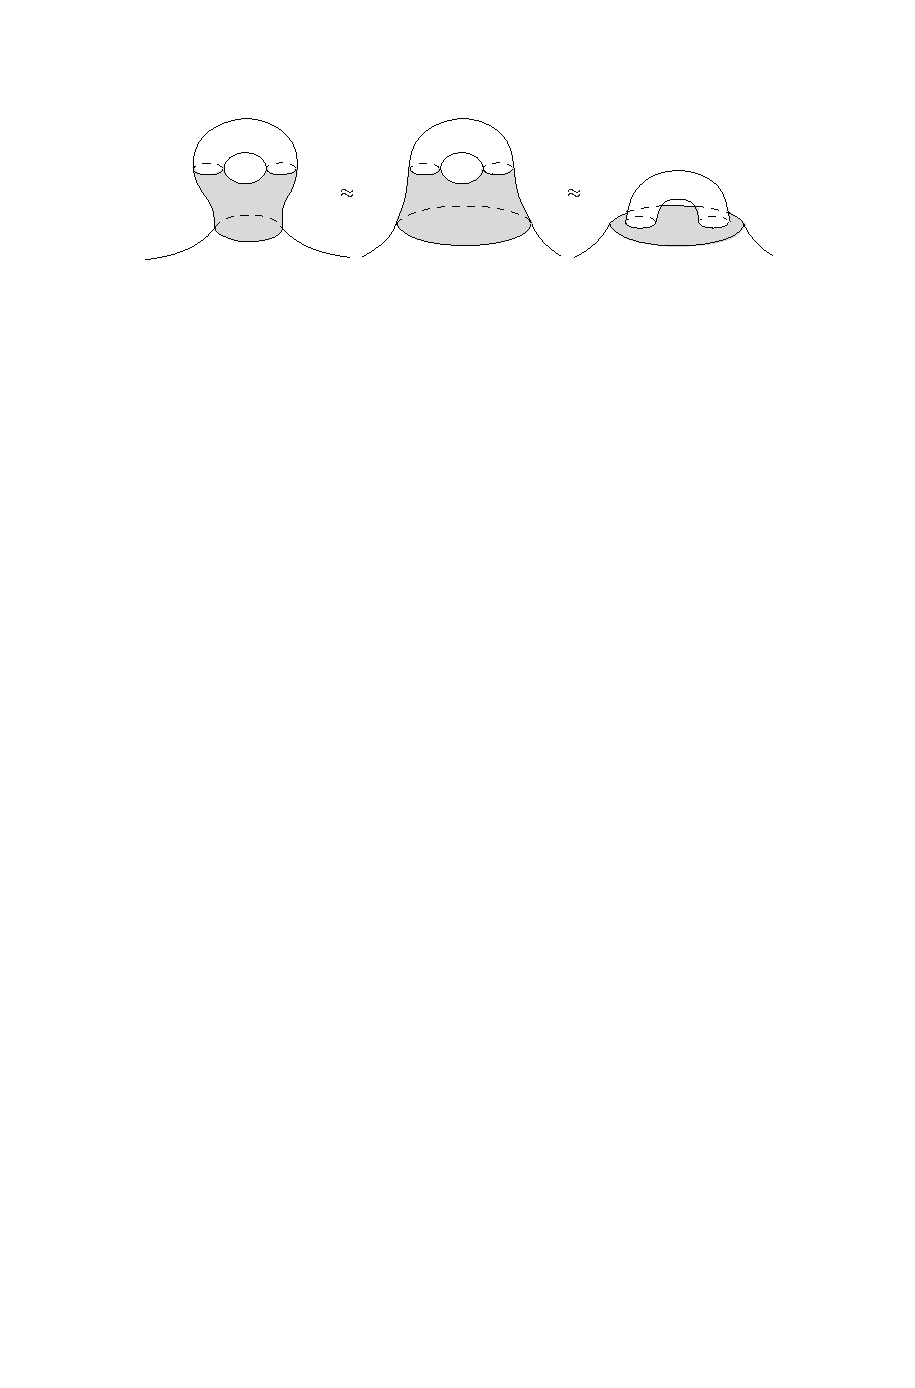
\includegraphics{handle.pdf}\]
\end{example}
\begin{example}
An $n$-fold connected sum $T^2\#T^2\#\cdots\#T^2$ is called an \textbf{$\bm{n}$-holed torus}. In view of the two preceding examples, it can also be considered as a sphere with $n$ handles attached.
\[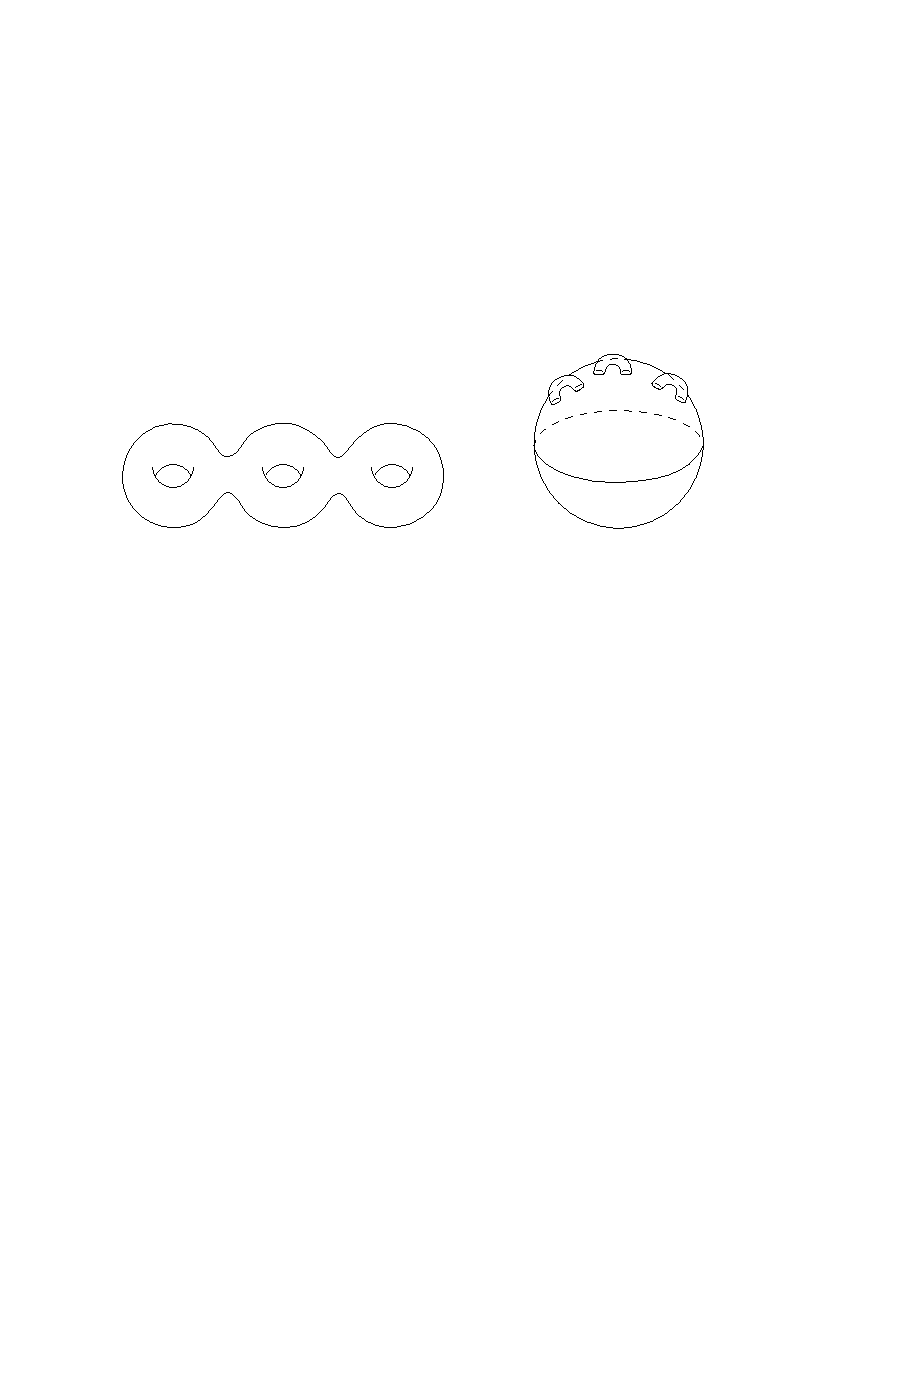
\includegraphics{n-tori.pdf}\]
\end{example}
\section{Polygonal Presentations of Surfaces}
For the classification theorem we need a uniform way to describe surfaces. We will represent all of our surfaces as quotients of $2n$-sided polygonal regions. Informally, we can describe any edge equivalence relation by labeling the edges with letters $a_1,\cdots,a_n$, and giving each edge an arrow pointing toward one of its vertices, in such a way that edges with the same label are to be identified, with the arrows indicating which way the vertices match up. With
each such labeling of a polygon we associate a sequence of symbols, obtained by
reading off the boundary labels counterclockwise from the top, and for each boundary label $a_i$, placing $a_i$ in the sequence if the arrow points counterclockwise and $a^{-1}_i$ if it points clockwise. For example, the equivalence relation on $I\times I$ that yields the torus might result in the sequence of symbols $aba^{-1}b^{-1}$.\par
Formally, given a set $S$, we define a \textbf{word} in $S$ to be an ordered $k$-tuple of symbols, each of the form $a$ or $a^{-1}$ for some $a\in S$. A polygonal presentation, written
\[\mathcal{P}=\langle S\mid W_1,\cdots,W_k\rangle\]
is a finite set $S$ together with finitely many words $W_1,\cdots,W_k$ in $S$ of length $3$ or more, such that every symbol in $S$ appears in at least one word. As a matter of notation, when the set $S$ is described by listing its elements, we leave out the braces surrounding the elements of $S$, and denote the words $W_i$ by juxtaposition. Thus, for example, the presentation with $S=\{a,b\}$ and the single word $W=(a,b,a^{-1},b^{-1})$ is written $\langle a,b\mid aba^{-1}b^{-1}\rangle$. We also allow as a special case any presentation in which $S$ has one element and there is a single word of length $2$. Except for renaming
the symbols, there are only four such: $\langle a\mid aa\rangle$, $\langle a\mid a^{-1}a^{-1}\rangle$, $\langle a\mid aa^{-1}\rangle$ and $\langle a\mid a^{-1}a\rangle$.\par
Any polygonal presentation $\mathcal{P}$ determines a topological space $|\mathcal{P}|$, called the \textbf{geometric realization} of $\mathcal{P}$, by the following recipe:
\begin{itemize}
\item For each word $W_i$, let $P_i$ denote the convex $k$-sided polygonal region in the plane that has its center at the origin, sides of length $1$, equal angles, and one vertex on the positive $y$-axis. (Here $k$ is the length of the word $W_i$.)
\item Define a one-to-one correspondence between the symbols of $W_i$ and the edges
of $P_i$ in counterclockwise order, starting at the vertex on the $y$-axis.
\item Let $\mathcal{P}|$ denote the quotient space of $\coprod_iP_i$ determined by identifying edges that have the same edge symbol, according to the affine homeomorphism that matches up the first vertices of those edges with a given label a and the last vertices of those with the corresponding label $a^{-1}$ (in counterclockwise order).
\end{itemize}
If $\mathcal{P}$ is one of the special presentations with a word of length $2$, we define $|\mathcal{P}|$ to be the sphere if the word is $aa^{-1}$ or $a^{-1}a$, and the projective plane if it is $aa$ or $a^{-1}a^{-1}$.\par
The interiors, edges, and vertices of the polygonal regions $P_i$ are called the \textbf{faces, edges, and vertices of the presentation}. The number of faces is the same as the number of words, and the number of edges is sum of the lengths of the words. For an edge labeled $a$, the \textbf{initial vertex} is the first one in counterclockwise order, and the \textbf{terminal vertex} is the other one; for an edge labeled $a^{-1}$, these definitions are reversed. In terms of our informal description above, if we label each edge with an arrow pointing counterclockwise when the symbol is $a$ and clockwise when it is $a^{-1}$, the arrow points from the initial vertex to the terminal vertex.\par
A polygonal presentation is called a surface presentation if each symbol $a\in S$
occurs exactly twice in $W_1,\cdots,W_k$ (counting either $a$ or $a^{-1}$ as one occurrence). By Proposition~\ref{polygonal quotient}, the geometric realization of a surface presentation is a compact surface.\par
If $X$ is a topological space and $\mathcal{P}$ is a polygonal presentation whose geometric realization is homeomorphic to $X$, we say that $\mathcal{P}$ is a presentation of $X$. A space that admits a presentation with only one face is connected, because it is homeomorphic to a quotient of a single connected polygonal region; with more than one face, it might or might not be connected.
\begin{example}
Here are some polygonal presentations of familiar surfaces
\begin{itemize}
\item The sphere: $\langle a\mid aa^{-1}\rangle$ or $\langle a,b\mid abb^{-1}a^{-1}\rangle$.
\item The torus: $\langle a,b\mid aaba^{-1}b^{-1}\rangle$.
\item The projective space: $\langle a,b\mid abab\rangle$.
\item The Klein bottle: $\langle a,b\mid abab^{-1}\rangle$.
\end{itemize}
\end{example}
For later use in proving the classification theorem, we need to develop some general rules for transforming polygonal presentations. If two presentations $\mathcal{P}_1$ and $\mathcal{P}_2$ have homeomorphic geometric realizations, we say that they are \textbf{topologically equivalent} and write $\mathcal{P}_1\approx\mathcal{P}_2$.\par
As a matter of notation, in what follows $S$ denotes any sequence of symbols; $a,b,c,a_1,a_2,\cdots$ denote any symbols from $S$ or their inverses; $e$ denotes any symbol not in $S$; and $W_1,W_2$ denote any words made from the symbols in $S$. Given two words $W_1,W_2$, the notation $W_1W_2$ denotes the word formed by concatenating $W_1$ and $W_2$. We adopt the convention that $(a^{-1})^{-1}=a$.\par
The following operations are called \textbf{elementary transformations} of a polygonal presentation.
\begin{itemize}
\item \textbf{Relabeling}: Changing all occurrences of a symbol $a$ to a new symbol not already in the presentation, interchanging all occurrences of two symbols $a$ and $b$, or interchanging all occurrences of $a$ and $a^{-1}$ for some $a\in S$.
\item \textbf{Subdividig}: Replacing every occurrence of $a$ by $ae$ and every occurrence of $a^{-1}$ by $e^{-1}a^{-1}$, where $e$ is a new symbol not already in the presentation.
\item \textbf{Consolidating}: If $a$ and $b$ always occur adjacent to each other either as $ab$ or $b^{-1}a^{-1}$, replacing every occurrence of $ab$ by $a$ and every occurrence of $b^{-1}a^{-1}$ by $a^{-1}$, provided that the result is one or more words of length at least $3$ or a single word of length $2$.
\item \textbf{Reflecting}: 
\[\langle S\mid a_1\cdots a_m,W_2,\cdot,W_k\rangle\mapsto\langle S\mid a_m^{-1}\cdots a_1^{-1},W_2,\cdots,W_k\rangle\]
\item \textbf{Rotating}: 
\[\langle S\mid a_1a_2\cdots a_m,W_2,\cdots,W_k\rangle\mapsto\langle S\mid a_2a_m\cdots a_1,W_2,\cdots,W_k\rangle\]
\item \textbf{Cutting}: If $W_1$ and $W_2$ both have length at least $2$,
\[\langle S\mid W_1W_2,W_3,\cdots,W_k\rangle\mapsto\langle S,e\mid W_1e,e^{-1}W_2, W_3,\cdots,W_k\rangle\]
\item \textbf{Pasting}:
\[\langle S,e\mid W_1e,e^{-1}W_2, W_3,\cdots,W_k\rangle\mapsto\langle S\mid W_1W_2,W_3,\cdots,W_k\rangle\]
\item \textbf{Folding}: If $W_1$ has length at least $3$,
\[\langle S,e\mid W_1ee^{-1},W_2, W_3,\cdots,W_k\rangle\mapsto\langle S\mid W_1,W_2,\cdots,W_k\rangle\]
We also allow $W_1$ to have length $2$, provided that the presentation has only one
word.
\item \textbf{Unfolding}:
\[\langle S\mid W_1,W_2,\cdots,W_k\rangle\mapsto\langle S,e\mid W_1ee^{-1},W_2, W_3,\cdots,W_k\rangle\]
\end{itemize}
\begin{figure}[htbp]
\centering
\begin{minipage}[b]{200pt}
\centering
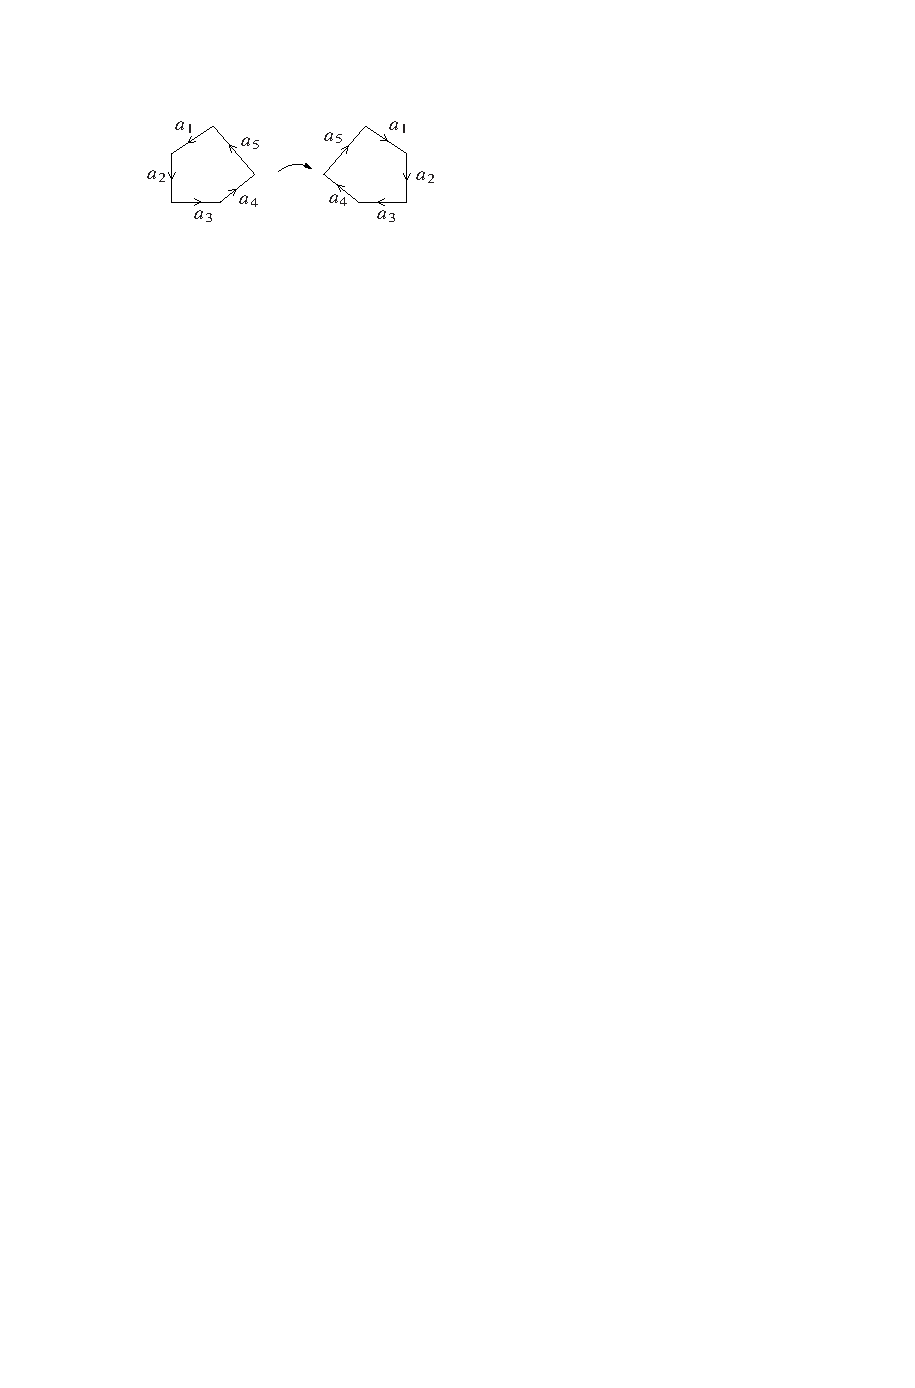
\includegraphics{reflecting.pdf}
\caption{Reflecting}
\end{minipage}
\hspace {20pt}
\begin{minipage}[b]{200pt}
\centering
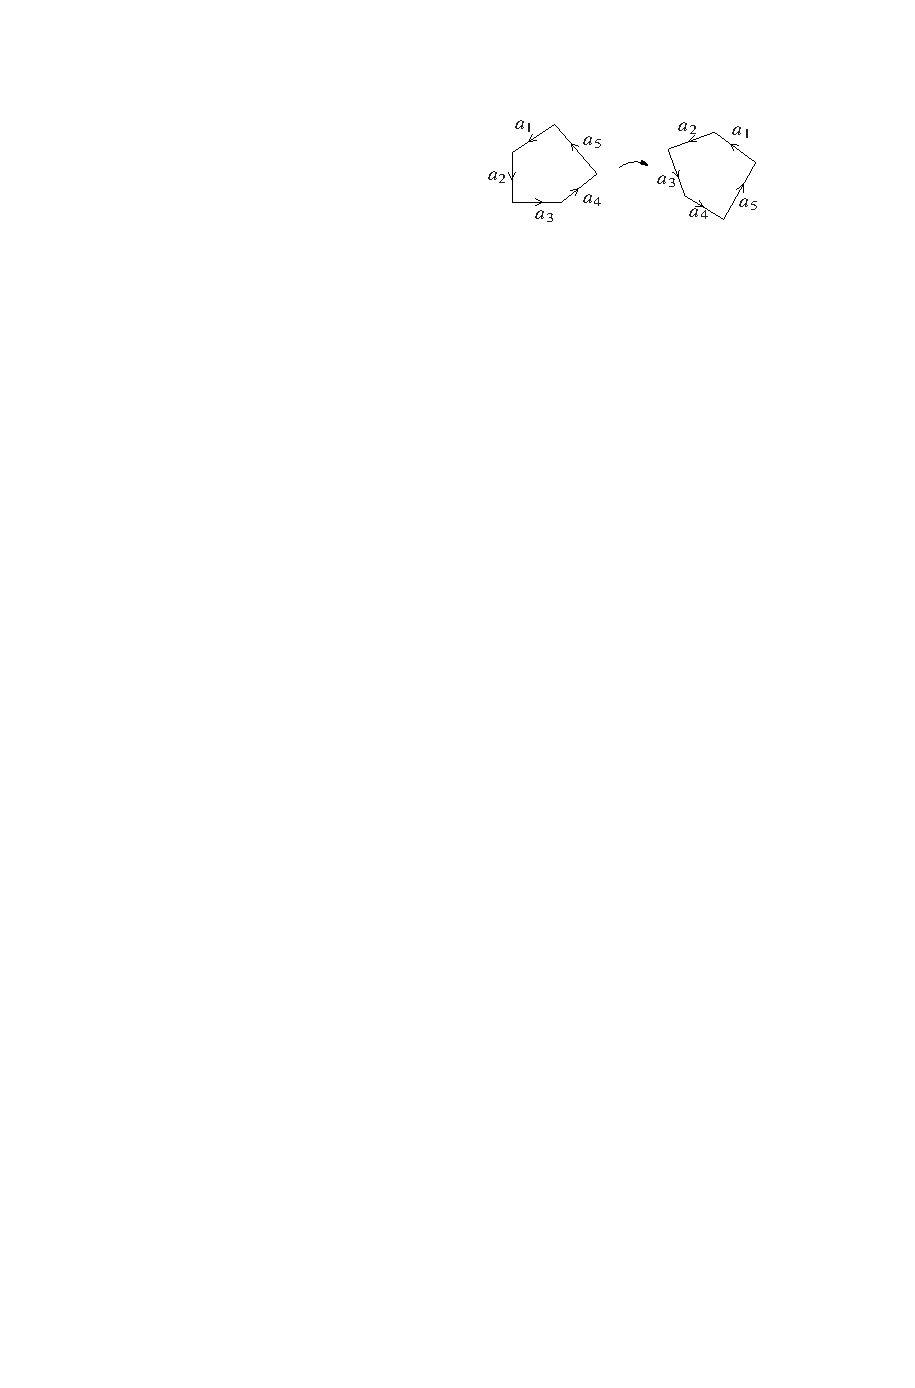
\includegraphics{rotating.pdf}
\caption{Rotating}
\end{minipage}
\end{figure}

\begin{figure}[htbp]
\centering
\begin{minipage}[t]{200pt}
\centering
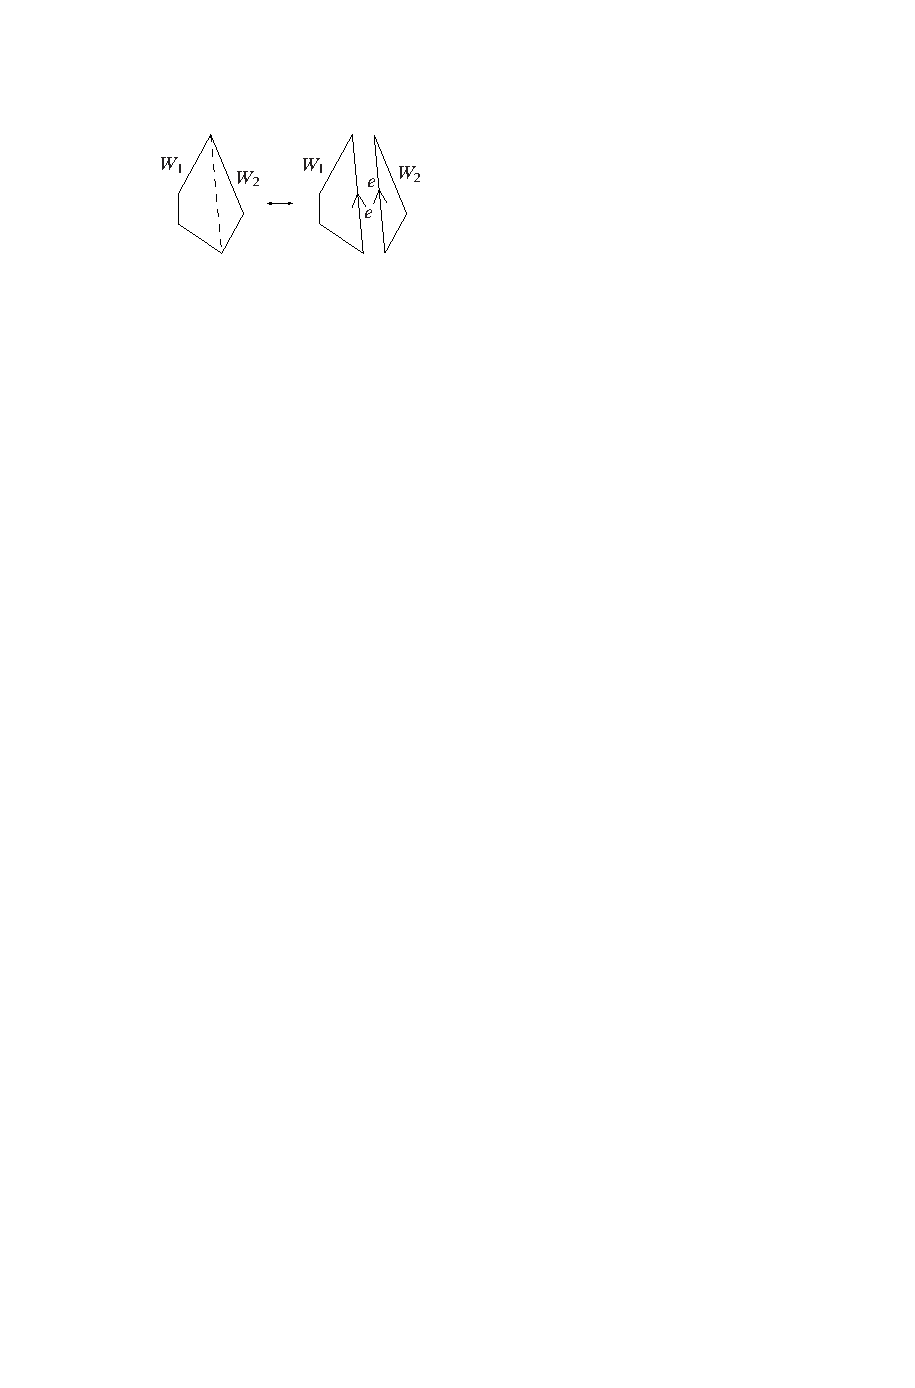
\includegraphics{cutting.pdf}
\caption{Cutting/Patsing}
\end{minipage}
\hspace {20pt}
\begin{minipage}[t]{200pt}
\centering
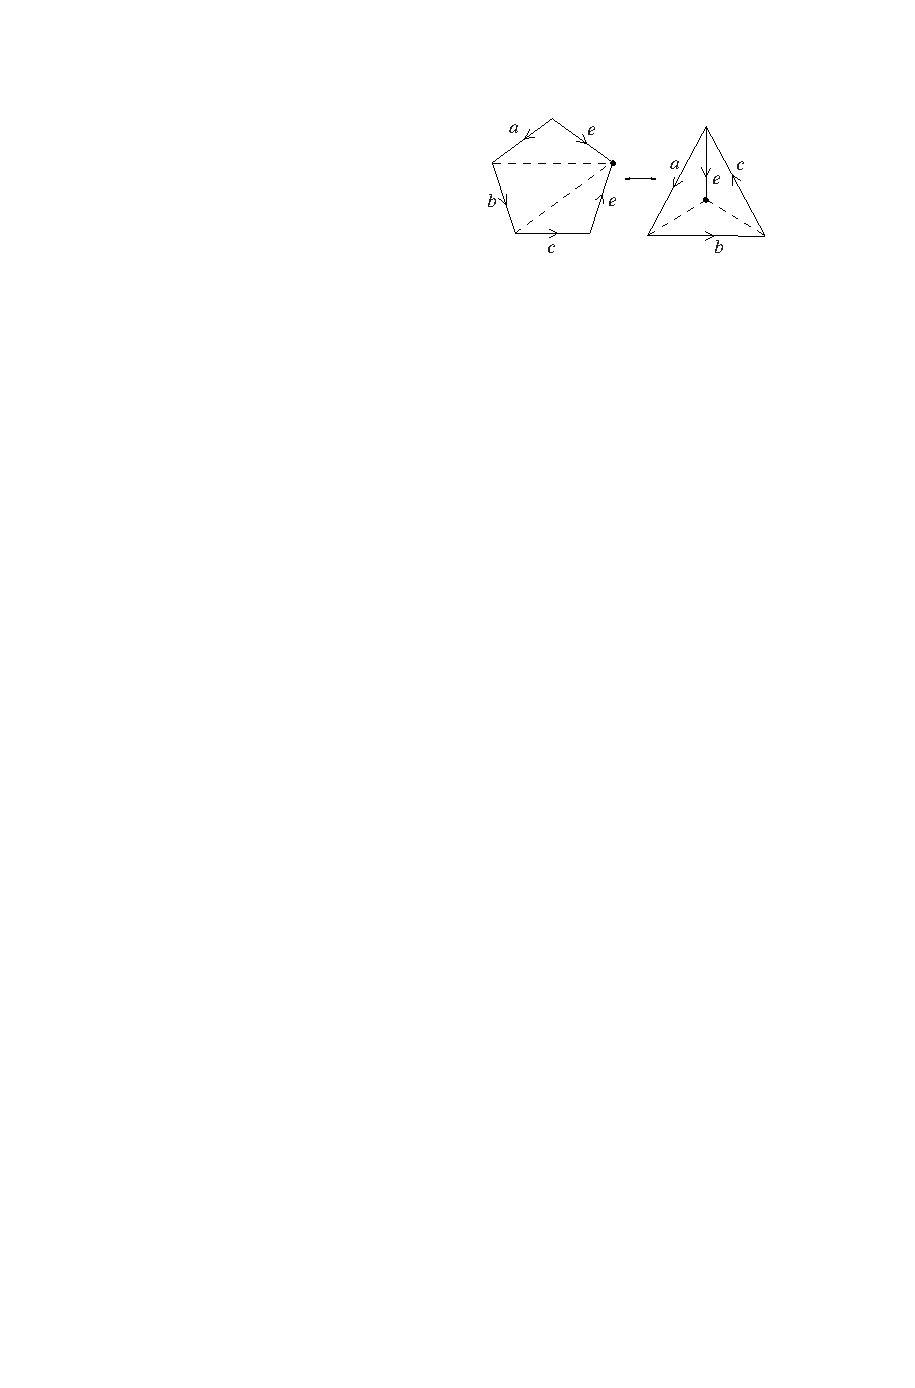
\includegraphics{folding.pdf}
\caption{Folding/Unfolding}
\end{minipage}
\end{figure}
\begin{proposition}
Each elementary transformation of a polygonal presentation produces a topologically equivalent presentation.
\end{proposition}
\begin{proof}
Clearly, subdividing and consolidating are inverses of each other, as are cutting/
pasting and folding/unfolding, so by symmetry only one of each pair needs to be proved. We demonstrate the techniques by proving the proposition for cutting
and folding.\par
To prove that cutting produces a homeomorphic geometric realization, let $P_1$ and
$P_2$ be convex polygonal regions labeled $W_1e$ and $e^{-1}W_2$, respectively, and let $P'$ be a convex polygonal region labeled $W_1W_2$. For the moment, let us 
assume that these are the only words in their respective presentations. Let $\pi:P_1\amalg P_2\to M$ and $\pi':P'\to M'$ denote the respective quotient maps. The 
line segment going from the terminal vertex of $W_1$ in $P_0$ to its initial vertex lies in $P_0$ by convexity; label this segment $e$. By the result of 
Exercise~\ref{extension maps on boundary of cell}, there is a continuous map $f:P_1\amalg P_2\to P'$ that takes each edge of $P_1$ or $P_2$ to the edge in $P'$ with the 
corresponding label, and whose restriction to each $P_i$ is a homeomorphism onto its image. By the closed map lemma, $f$ is a quotient map. Since $f$ identifies the two 
edges labeled $e$ and $e^{-1}$ but nothing else, the quotient maps $\pi'\circ f$ and $\pi$ make precisely the same identifications, so their quotient spaces are 
homeomorphic. If there are other words $W_3,\cdots,W_k$, we just extend $f$ by declaring it to be the identity on their respective polygonal regions and proceed as 
above.\par
For folding, as before we can ignore the additional words $W_2,\cdots,W_k$. If $W_1$ has length $2$, we can subdivide to lengthen it, then perform the folding 
operation, and then consolidate, so we assume that $W_1$ has length at least $3$. Assume first that $W_1=abc$ has length exactly $3$. Let $P$ and $P'$ be convex 
polygonal regions with edge labels $abcee^{-1}$ and $abc$, respectively, and let $\pi:P\to M$, $\pi':P'\to M'$ be the quotient maps. Adding edges turns $P$ and $P'$ 
into polyhedra of Euclidean simplicial complexes, and there is a unique simplicial map $f:P\to P'$ that takes each edge of $P$ to the edge of $P'$ with the same label. 
As before, $\pi'\circ f$ and $\pi$ are quotient maps that make the same identifications, so their quotient spaces are homeomorphic.\par
If $W_1$ has length $4$ or more, we can write $W_1=Xbc$ for some $X$ of length at
least $2$. Then we cut along a new edge $a$ to obtain
\[\langle S,b,c,e\mid Xbcee^{-1}\rangle\approx\langle S,a,b,c,e\mid Xa^{-1}, abcee^{-1}\rangle\]
and proceed as before.
\end{proof}
Next we need to find standard polygonal presentations for connected sums. The
key is the following proposition.
\begin{proposition}
Let $M_1$ and $M_2$ be surfaces that admit presentations $\langle S_1\mid W_1\rangle$ and $\langle S_2\mid W_2\rangle$, respectively, in which $S_1$ and $S_2$ are disjoint sets and each presentation has a single face. Then $\langle S_1,S_2\mid W_1W_2\rangle$ is a presentation of a connected sum $M_1\#M_2$. $($Here $W_1W_2$ denotes the word formed by concatenating $W_1$ and $W_2$.$)$
\end{proposition}
\begin{proof}
Consider the presentation $\langle S_1,a,b,c\mid W_1c^{-1}b^{-1}a^{-1},abc\rangle$. Pasting along $a$ and folding twice, we see that this presentation is equivalent to $\langle S_1,W_1\rangle$ and therefore is a presentation of $M_1$. Let $B_1$ denote the image in $M_1$ of the interior of the polygonal region bounded by triangle $abc$. We will show below that $B_1$ is a regular coordinate disk in $M_1$. Assuming this, it follows immediately that the geometric realization of $\langle S_1,a,b,c\mid W_1c^{-1}b^{-1}a^{-1}\rangle$ is homeomorphic to $M_1\setminus B_1$ (which we denote by $M'_1$), and $\partial B_1$ is the image of the edges $c^{-1}b^{-1}a^{-1}$. A similar argument shows that  is a presentation of $M_2$ with a coordinate disk removed (denoted by $M'_2$ ). Therefore, $\langle S_1,S_2,a,b,c\mid abcW_2\rangle$ is a presentation of $M'_1\amalg M'_2$ with the boundaries of the respective disks identified, which is $M_1\#M_2$. Pasting along a and folding twice, we arrive at the presentation $\langle S_1,S_2\mid W_1W_2\rangle$.\par
It remains only to show that $B_1$ is a regular coordinate disk in $M_1$, which is to say that it has an open disk neighborhood in which $\widebar{B}_1$ corresponds to a smaller closed disk. One way to see this is suggested: let $P_1$, $Q$, and $P'_1$ be convex polygonal regions with edges labeled by the words $W_1c^{-1}b^{-1}a^{-1}$, $abc$, and $W_1$, respectively. Triangulate the polygonal regions, we obtain a simplicial map $f:P_1\amalg Q\to P'_1$ that takes $Q$ to a small triangle $Q'\sub P'_1$ sharing one vertex $v$ in common with $P'_1$. The composition $P_1\amalg Q\to P'_1\to M_1$ respects the identifications made by the quotient map $P'_1\amalg Q\to M_1$, so it descends to a homeomorphism of $M_1$ taking $B_1$ to the image of $Q'$. Now look back at the proof in Proposition~\ref{polygonal quotient} that the quotient space of a surface presentation is a manifold. In constructing a Euclidean neighborhood of a vertex point, we assembled wedges at the various vertices into a coordinate disk. Applying that construction to the vertex $v$, $Q'$ is taken to a set that is homeomorphic to a closed disk in the plane, and it is an easy matter to extend that homeomorphism to a slightly larger open disk.
\end{proof}
\begin{example}
Using the preceding proposition, we can augment our list of presentations of known surfaces as follows. To streamline the list of surfaces, we interpret a connected sum of one torus to mean simply $T^2$ itself, and similarly for $P^2$.
\begin{itemize}
\item Sphere:
\[\langle a\mid aa^{-1}\rangle\]
\item Connected sum of $n\geq 1$ tori:
\[\langle a_1,b_1,\cdots,a_n,b_n\mid a_1b_1a_1^{-1}b_1^{-1}\cdots a_nb_na_n^{-1}b_n^{-1}\rangle\]
\item Connected sum of $n\geq 1$ projective plane:
\[\langle a_1,\cdots,a_n\mid a_1a_1\cdots a_na_n\rangle\]
\end{itemize}
We call these the standard presentations of these surfaces.
\end{example}
\section{The Classification Theorem}
\begin{proposition}
Every compact surface admits a polygonal presentation.
\end{proposition}
\begin{proof}
Let $M$ be a compact surface. It follows from Theorem~\ref{two mani triangulate} that $M$ is homeomorphic to the polyhedron of a $2$-dimensional simplicial complex $K$, in which each $1$-simplex is a face of exactly two $2$-simplices. From this complex, we can construct a surface presentation $\mathcal{P}$ with one word of length $3$ for each $2$-simplex, and with edges having the same label if and only if they correspond to the same $1$-simplex. We wish to show that the geometric realization of $\mathcal{P}$ is homeomorphic to that of $K$. If $P=P_1\amalg\cdots\amalg P_k$ denotes the disjoint union of the $2$-simplices of $K$, then we have two quotient maps $\pi_K:P\to|K|$ and $\pi_\mathcal{P}:P\to|\mathcal{P}|$, so it suffices to show that they make the same identifications. Both quotient maps are injective in the interiors of the $2$-simplices, both make the same identifications of edges, and both identify vertices only with other vertices.\par
To complete the proof, we need to show that $\pi_K$, like $\pi_\mathcal{P}$, identifies vertices only when forced to do so by the relation generated by edge identifications. To prove this, suppose $v\in K$ is any vertex. It must be the case that $v$ belongs to some $1$-simplex, because otherwise it would be an isolated point of $|K|$, contradicting the fact that $|K|$ is a $2$-manifold. Theorem~\ref{two mani triangulate} guarantees that this $1$-simplex is a face of exactly two $2$-simplices. Let us say that two $2$-simplices $\sigma$, $\sigma'$ containing $v$ are \textbf{edge-connected} at $v$ if there is a sequence $\sigma=\sigma_1,\cdots,\sigma_k=\sigma'$ of $2$-simplices containing $v$ such that $\sigma_i$ shares an edge with $\sigma_{i+1}$ for each $i=1,\cdots,k-1$. Clearly edge-connectedness is an equivalence relation on the set of $2$-simplices containing $v$, so to prove the claim it suffices to show that there is only one equivalence class. If this is not the case, we can group the $2$-simplices containing $v$ into two disjoint sets $\{\sigma_1,\cdots,\sigma_k\}$ and $\{\tau_11,\cdots,\tau_k\}$, such that any $\sigma_i$ and $\sigma_j$ are edge-connected to each other, but no $\sigma_i$ is edge-connected to any $\tau_j$. Let $\eps$ be chosen small enough that $\B(v,\eps)$ intersects only those simplices that contain $v$. Then $\B(v,\eps)\cap|K|$ is an open subset of $|K|$ and thus a $2$-manifold, so $v$ has a neighborhood $W\sub\B(v,\eps)\cap|K|$ that is homeomorphic to $\R^2$. It follows that $W\setminus\{v\}$ is connected. However, if we set
\[U=W\cap(\sigma_1\cup\cdots\cup\sigma_k)\setminus\{v\},\quad V=W\cap(\tau_1\cup\cdots\tau_m)\setminus\{v\}\]
then $U$ and $V$ are both open in $|K|$ because their intersection with each simplex is open in the simplex, and $W=U\cup V$ is a disconnection of $W$. This is a contradiction.
\end{proof}
\begin{lemma}
The Klein bottle is homeomorphic to $\P^2\#\P^2$.
\end{lemma}
\begin{proof}
By a sequence of elementary transformations, we find that the Klein bottle has the following presentations
\begin{align*}
\langle a,b\mid abab^{-1}\rangle=\langle a,b,c\mid abc,c^{-1}ab^{-1}\rangle=\langle a,b,c\mid bca,a^{-1}cb\rangle=\langle b,c\mid bccb\rangle=\langle b,c\mid ccbb\rangle
\end{align*}
\end{proof}
\begin{lemma}\label{T^2 sum P^2}
The connected sum $T^2\#\P^2$ is homeomorphic to $\P^2\#\P^2\#\P^2$.
\end{lemma}
\begin{proof}
Start with $\langle a,b,c\mid abab^{-1}cc\rangle$, which is a presentation of $K\#\P^2$,
and therefore by the preceding lemma is a presentation of $\P^2\#\P^2\#\P^2$. Following Figure~\ref{P^2sumT^2}, we cut along $d$, paste along $c$, cut along $e$, and paste along $b$, rotating and reflecting as necessary, to obtain $\langle a,d,e\mid a^{-1}d^{-1}adee\rangle$, which is a presentation of $T^2\#\P^2$.
\begin{figure}[!h]
\centering
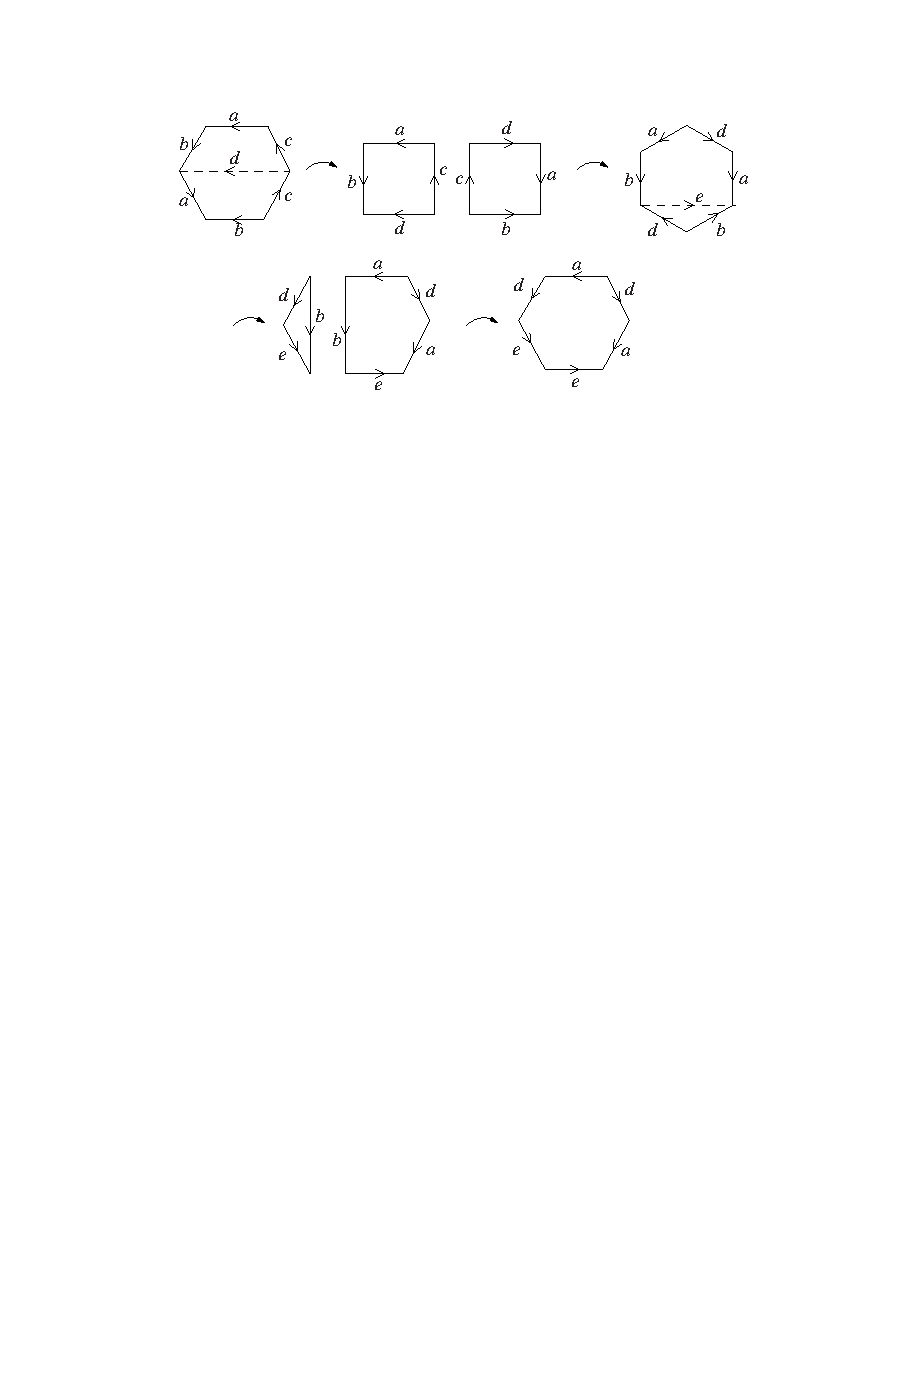
\includegraphics{T^2sumP^2}
\caption{Transforming $\P^2\#\P^2\#\P^2$ to $T^2\#\P^2$}
\label{P^2sumT^2}
\end{figure}
\end{proof}
\begin{theorem}[\textbf{Classification of Compact Surfaces}]
Every nonempty, compact, connected $2$-manifold is homeomorphic to one of the following:
\begin{itemize}
\item[$(a)$] The sphere $S^2$.
\item[$(b)$] A connected sum of one or more copies of $T^2$.
\item[$(c)$] A connected sum of one or more copies of $\P^2$.
\end{itemize}
\end{theorem}
\begin{proof}
Let us say that a pair of edges that are to be identified are \textbf{complementary} if they appear in the presentation as both $a$ and $a^{-1}$, and twisted if they appear as $a,\cdots,a$ or as $a^{-1},\cdots,a^{-1}$.\par
For a compact surface $M$, we list a few facts:
\begin{itemize}
\item $M$ admits a presentation with only one face.
\item Either $M$ is homeomorphic to the sphere, or $M$ admits a presentation in which there are no adjacent complementary pairs.
\item $M$ admits a presentation in which all twisted pairs are adjacent. In fact, a word $VaWa$ can be transformed into $VW^{-1}bb$:
\[\langle VaWa\rangle=\langle Vab,b^{-1}Wa\rangle=\langle bVa,a^{-1}W^{-1}b\rangle=\langle bVW^{-1}b\rangle=\langle VW^{-1}bb\rangle\]
\item $M$ admits a presentation in which all vertices are identified to a single point.
\item If the presentation has any complementary pair $a,a^{-1}$, then it has
another complementary pair $b,b^{-1}$ that occurs intertwined with the first, as in $a,\cdots,b,\cdots,a^{-1},\cdots,b^{-1}$ (occurs in this order).
\item $M$ admits a presentation in which all intertwined complementary pairs occur together with no other edges intervening: $aba^{-1}b^{-1}$:
\begin{align*}
\langle WaXbYa^{-1}Zb^{-1}\rangle&=\langle WaXc,c^{-1}bYa^{-1}Zb^{-1}\rangle=\langle XcWa,a^{-1}Zb^{-1}c^{-1}bY\rangle\\
&=\langle XcWZb^{-1}c^{-1}bY\rangle=\langle c^{-1}bYXcWZb^{-1}\rangle\\
&=\langle c^{-1}bYXcd,d^{-1}WZb^{-1}\rangle=\langle YXcdc^{-1}b,b^{-1}d^{-1}WZ\rangle\\
&=\langle YXcdc^{-1}d^{-1}WZ\rangle=\langle YXcdc^{-1}d^{-1}WZ\rangle\\
&=\langle WZYXcdc^{-1}d^{-1}\rangle
\end{align*}
\item $M$ is homeomorphic to either a connected sum of one or more tori or a connected sum of one or more projective planes. In fact, the only problem occurs where the presentation contains both twisted
and complementary pairs. That is, it is a connect sum of toris and projective planes. Lemma~\ref{T^2 sum P^2} eliminates a projective space, hence gives the claim.
\end{itemize}
\end{proof}
\section{The Euler Characteristic}
One of the oldest results in the theory of surfaces is Euler's formula: if $P\sub\R^3$ is a compact polyhedral surface that is the boundary of a convex open subset, and $P$ has
$F$ faces, $E$ edges, and $V$ vertices, then $V-E+F=2$. This quantity has a natural generalization to arbitrary finite CW complexes: if $X$ is a finite CW complex of
dimension $n$, we define the \textbf{Euler characteristic} of $X$, denoted by $\chi(X)$, by
\[\chi(X):=\sum_{k=0}^{n}(-1)^kn_k\]
As a matter of fact, the Euler characteristic can be computed by homology, hence is a topological invariant for finite CW complexes.
\begin{proposition}
The Euler characteristic of a polygonal presentation is unchanged by elementary transformations.
\end{proposition}
\begin{proof}
It is immediate that relabeling, rotating, and reflecting do not change the Euler characteristic of a presentation, because they leave the numbers of $0$-cells, $1$-cells, and $2$-cells individually unchanged. For the other transformations, we need only check that the changes to these three numbers cancel out. Subdividing increases both the number of $1$-cells and the number of $0$-cells by one, leaving the number of $2$-cells unchanged. Cutting increases both the number of $1$-cells and the number of $2$-cells by one, and leaves the number of $0$-cells unchanged. Unfolding increases the number of $1$-cells and the number of $0$-cells by one, and leaves the number of $2$-cells unchanged. Finally, consolidating, pasting, and folding leave the Euler characteristic unchanged, since they are the inverses of subdividing, cutting, and
unfolding, respectively.
\end{proof}
\begin{proposition}
The Euler characteristic of a standard surface presentation is equal to
\begin{itemize}
\item[$(a)$] $2$ for the sphere.
\item[$(b)$] $2-2n$ for the connected sum of $n$ tori.
\item[$(c)$] $2-n$ for the connected sum of $n$ projective planes.
\end{itemize}
\end{proposition}
\section{Orientability}
The \textbf{M\"obius band} is the famous topological space obtained from a rectangle by
pasting two opposite sides together after a half-twist. Formally, we define it to be
the geometric realization of the following polygonal presentation:
\[\langle a,b,c\mid abcb\rangle\]
It is a $2$-dimensional manifold with boundary, and it has a \textit{twisted boundary}.\par
Motivated by this example, let us say that a surface presentation $\mathcal{P}$ is oriented
if it has no twisted edge pairs. A compact surface is said to be \textbf{orientable} if it admits an oriented presentation.
\begin{proposition}
A compact surface is orientable if and only if it is homeomorphic to the sphere or a connected sum of one or more tori.
\end{proposition}
Because of this result, the connected sum of $n$ tori is also known as the \textbf{orientable surface of genus $\bm{n}$}, and the connected sum of $n$ projective planes is called the \textbf{nonorientable surface of genus $\bm{n}$}. By convention, the sphere is the (unique, orientable) \textbf{surface of genus $\bm{0}$}.
\section{Exercise}
\begin{exercise}
Show that a connected sum of one or more projective planes contains a subspace that is homeomorphic to the M\"obius band.
\end{exercise}
\begin{exercise}
Note that both a disk and a M\"obius band are manifolds with boundary, and both boundaries are homeomorphic to $S^1$. Show that it is possible to obtain a space homeomorphic to a projective plane by attaching a disk to a M\"obius band along their boundaries.
\end{exercise}
\begin{proof}
The figure 
\[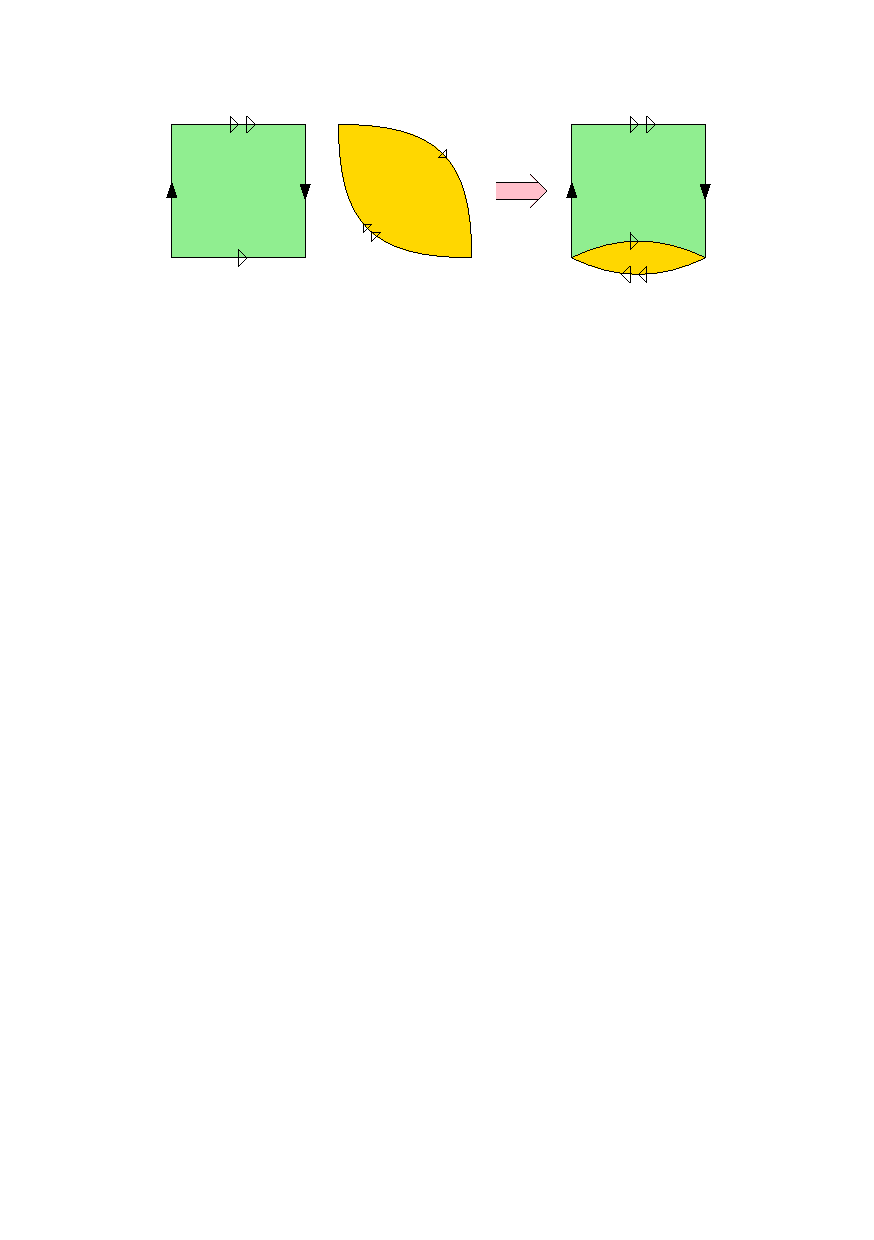
\includegraphics{Mobious+disk}\]
gives the ideal.
\end{proof}
\begin{exercise}
Show that the Klein bottle is homeomorphic to a quotient obtained by attaching two M\"obius bands together along their boundaries.
\end{exercise}
\begin{proof}
This is a diagram of the Klein bottle, note that the diagonal lines divide it into $2$ M\"obius strips 
sharing a boundary:
\[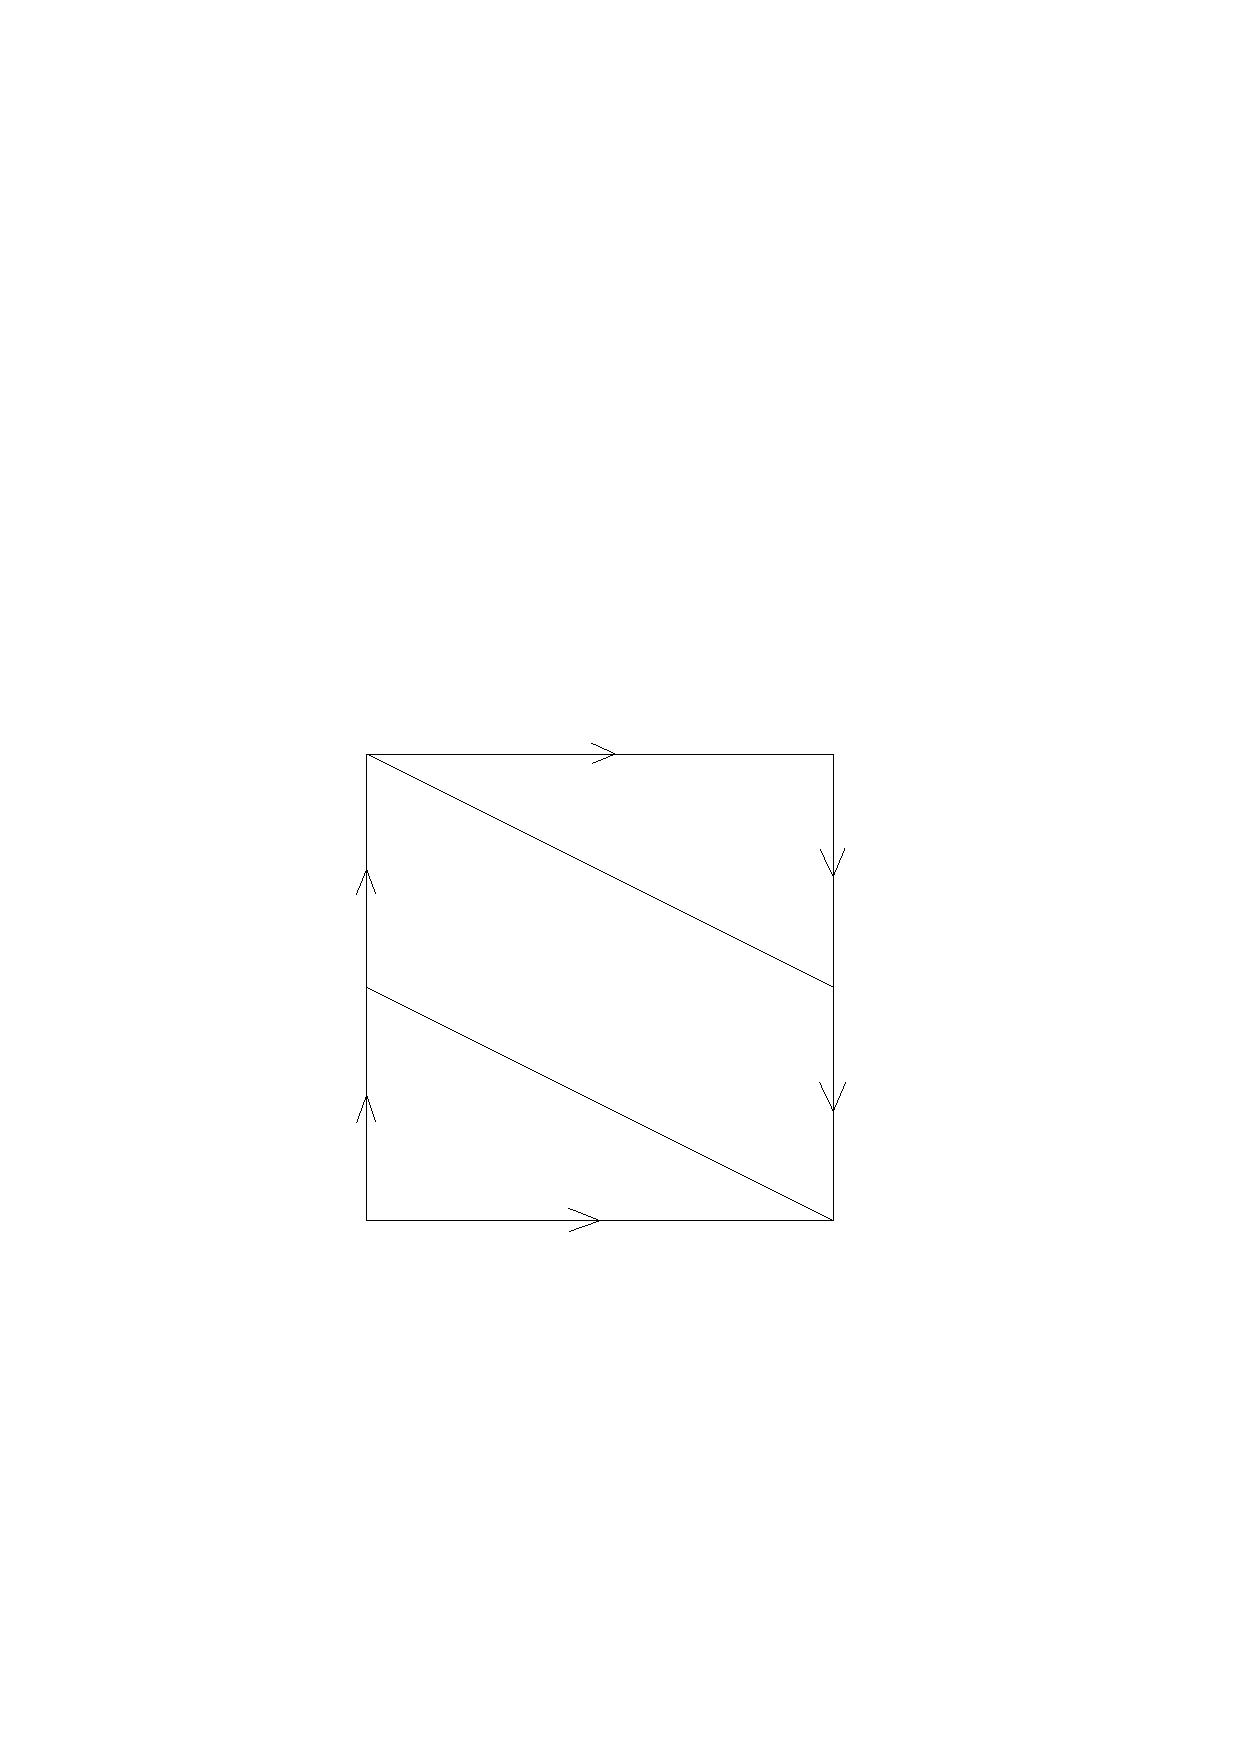
\includegraphics[width=0.25\textwidth]{Klein-Mobious}\]
Therefore the claim follows.
\end{proof}
\begin{exercise}
Suppose $M$ is a compact, connected $2$-manifold that contains a subset $B\sub M$ that is homeomorphic to the M\"obius band. Show that there is a compact $2$-manifold $M'$ such that $M$ is homeomorphic to a connected sum $M'\#\P^2$.
\end{exercise}
\begin{proof}
$M$ has a twisted edge, so it is a connect sum of projective planes.
\end{proof}
\begin{exercise}
Show that every compact $2$-manifold with boundary is homeomorphic to a compact $2$-manifold with finitely many open cells removed.
\end{exercise}
\begin{proof}
The boundary is a compace $1$-manifold, so each of its connected component is homeomorphic to the circle. And it has only finitely many connected component, so is homeomorphic to a disjoint union of circles. We attach disks along the boundary to get a compact $2$-manifold. (Proposition~\ref{adju mani})
\end{proof}
\begin{exercise}
For each of the following surface presentations, compute the Euler characteristic and determine which of our standard surfaces it represents.
\begin{itemize}
\item[$(a)$]$\langle a,b,c\mid abacb^{-1}c^{-1}\rangle$ 
\item[$(b)$]$\langle a,b,c\mid abca^{-1}b^{-1}c^{-1}\rangle$ 
\item[$(c)$]$\langle a,b,c,d,e,f\mid abc,bde,c^{-1}df,e^{-1}fa\rangle$ 
\end{itemize}
\end{exercise}
\begin{proof}
\mbox{}
\begin{itemize}
\item $\chi=2-3=-1$, so the surface is $\P^2\#\P^2\#\P^2$.
\item $\chi=3-3=0$. The surface is $T^2$.
\item $\chi(M_1\#M_2)=\chi(M_1)+\chi(M_2)-2$. The presentation has $3$ vertices, $6$ edges, $1$ face. So $\chi=-2$. And the surface is $\P^2\#\P^2\#\P^2\#\P^2$.
\end{itemize}
\end{proof}
\begin{remark}
If the polygonal presentation contains only one word, the following algorithm works:
\begin{itemize}
\item Add vertex symbols. Then, for each pair of edges with the same edge symbol, build one set containing the two initial vertices and one set containing the two terminal vertices.
\item Build the union of all vertex sets that have at least one vertex in common until all resulting sets are disjoint.
\item The number of vertices is the number of disjoint sets obtained in step 2. The number of edges is the number of different edge symbols and the number of faces is one.
\end{itemize}
\end{remark}